\documentclass[dvisvgm,multi=true]{standalone}
\usepackage{mathmlcoresvg}
\begin{document}

%<figcaption><span>Figure 5: </span>Base size, size variants and glyph assembly for the left brace</figcaption>
  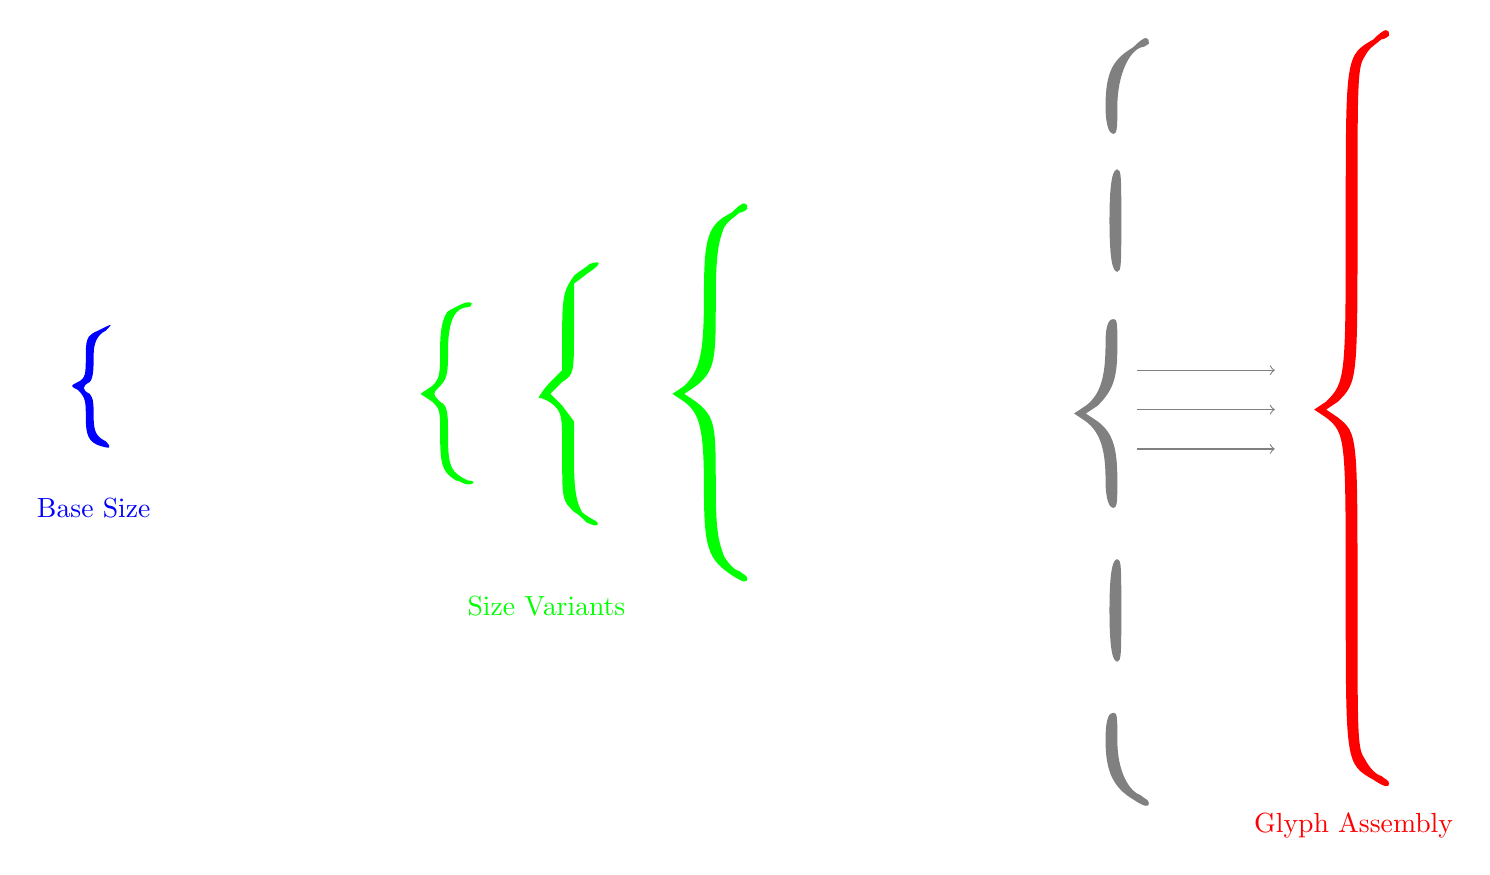
\begin{tikzpicture}[yscale=-1]

    \begin{scope}[xscale=.05,yscale=.05]

      \fill[blue] (11,109) .. controls (9,108) and (8,107) .. (8,102) .. controls (8,98) and (8,97) .. (6,95) .. controls (4,94) and (4,94) .. (6,93) .. controls (8,92) and (8,91) .. (8,86) .. controls (8,81) and (9,81) .. (11,80) .. controls (15,78) and (15,78) .. (13,80) .. controls (11,81) and (10,83) .. (10,86) .. controls (10,89) and (10,92) .. (9,93) .. controls (7,94) and (7,95) .. (9,96) .. controls (10,97) and (10,99) .. (10,102) .. controls (10,106) and (11,107) .. (13,108) .. controls (15,110) and (14,110) .. (11,109);
      \draw[blue] (10,120) node[below]{Base Size};

      \fill[green] (172,142) .. controls (166,138) and (165,135) .. (165,120) .. controls (165,105) and (164,101) .. (160,98) -- (157,96) -- (160,94) .. controls (164,90) and (165,86) .. (165,71) .. controls (165,56) and (166,53) .. (172,50) .. controls (175,47) and (176,47) .. (176,49) .. controls (176,49) and (175,50) .. (174,50) .. controls (173,51) and (171,52) .. (170,54) .. controls (169,57) and (168,59) .. (168,72) .. controls (168,87) and (168,90) .. (163,94) -- (160,96) -- (163,98) .. controls (168,102) and (168,104) .. (168,120) .. controls (168,132) and (169,134) .. (170,137) .. controls (171,139) and (173,141) .. (174,141) .. controls (175,142) and (176,142) .. (176,143) .. controls (176,144) and (175,144) .. (172,142);
      \fill[green] (136,129) .. controls (135,129) and (134,127) .. (132,126) .. controls (129,123) and (129,123) .. (129,112) .. controls (129,102) and (129,101) .. (127,99) .. controls (126,98) and (124,97) .. (123,97) .. controls (123,97) and (124,95) .. (126,93) -- (129,90) -- (129,79) .. controls (129,70) and (130,69) .. (132,66) .. controls (133,65) and (135,64) .. (136,63) .. controls (139,62) and (139,63) .. (136,65) -- (132,68) -- (132,79) .. controls (132,91) and (132,91) .. (129,93) -- (126,96) -- (129,99) -- (132,103) -- (132,113) .. controls (132,122) and (133,124) .. (134,126) .. controls (135,127) and (137,128) .. (137,128) .. controls (139,129) and (138,130) .. (136,129);
      \fill[green] (102,118) .. controls (99,116) and (98,115) .. (98,107) .. controls (98,100) and (98,100) .. (96,98) -- (93,96) -- (96,94) .. controls (98,92) and (98,91) .. (98,84) .. controls (98,79) and (99,76) .. (100,75) .. controls (102,74) and (105,72) .. (106,73) .. controls (106,73) and (106,74) .. (105,74) .. controls (102,74) and (100,77) .. (100,85) .. controls (100,90) and (100,92) .. (98,94) .. controls (96,96) and (96,96) .. (98,98) .. controls (100,99) and (100,101) .. (100,107) .. controls (100,115) and (101,116) .. (105,118) .. controls (107,118) and (107,119) .. (105,119) .. controls (104,119) and (103,118) .. (102,118);
      \draw[green] (125,145) node[below]{Size Variants};

      \fill[gray] (274,199) .. controls (269,196) and (267,192) .. (267,184) .. controls (267,178) and (268,177) .. (269,177) .. controls (270,177) and (270,178) .. (270,184) .. controls (270,192) and (273,197) .. (276,198) .. controls (277,199) and (278,199) .. (278,200) .. controls (278,201) and (277,201) .. (274,199);
      \fill[gray] (268,151) .. controls (268,140) and (269,138) .. (270,138) .. controls (271,138) and (271,140) .. (271,151) .. controls (271,162) and (271,164) .. (270,164) .. controls (269,164) and (268,162) .. (268,151);
      \fill[gray] (267,118) .. controls (267,111) and (266,106) .. (262,103) -- (259,101) --  (262,99) .. controls (266,96) and (267,91) .. (267,83) .. controls (267,78) and (268,77) .. (269,77) .. controls (270,77) and (270,78) .. (270,84) .. controls (270,92) and (269,95) .. (265,99) -- (262,101) -- (265,103) .. controls (269,106) and (270,110) .. (270,118) .. controls (270,123) and (270,125) .. (269,125) .. controls (268,125) and (267,123) .. (267,118);
      \fill[gray](268,52) .. controls (268,41) and (269,39) .. (270,39) .. controls (271,39) and (271,41) .. (271,52) .. controls (271,63) and (271,65) .. (270,65) .. controls (269,65) and (268,63) .. (268,52);
      \fill[gray] (267,23) .. controls (267,14) and (269,11) .. (274,8) .. controls (277,5) and (278,5) .. (278,7) .. controls (278,7) and (277,8) .. (276,8) .. controls (273,9) and (270,15) .. (270,23) .. controls (270,28) and (270,30) .. (269,30) .. controls (268,30) and (267,28) .. (267,23);

      \draw[->,color=gray] (275,90) -- (310,90);
      \draw[->,color=gray] (275,100) -- (310,100);
      \draw[->,color=gray] (275,110) -- (310,110);

      \fill[red] (335,194) .. controls (328,190) and (328,190) .. (328,148) .. controls (328,107) and (328,106) .. (323,102) -- (320,100) -- (323,98) .. controls (328,93) and (328,92) .. (328,51) .. controls (328,10) and (328,10) .. (335,6) .. controls (338,3) and (339,3) .. (339,5) .. controls (339,5) and (338,6) .. (337,6) .. controls (336,7) and (334,8) .. (333,10) .. controls (331,13) and (331,15) .. (331,52) .. controls (331,93) and (331,93) .. (326,98) -- (323,100) -- (326,102) .. controls (331,106) and (331,106) .. (331,148) .. controls (331,185) and (331,186) .. (333,189) .. controls (334,191) and (336,193) .. (337,193) .. controls (338,194) and (339,194) .. (339,195) .. controls (339,196) and (338,196) .. (335,194) -- cycle;
      \draw[red] (330,200) node[below]{Glyph Assembly};
    \end{scope}
    \end{tikzpicture}
\end{document}
